%###############################################################################
%# N1 - Manual - Instruction set                                               #
%###############################################################################
%#    Copyright 2018 Dirk Heisswolf                                            #
%#    This file is part of the N1 project.                                     #
%#                                                                             #
%#    N1 is free software: you can redistribute it and/or modify               #
%#    it under the terms of the GNU General Public License as published by     #
%#    the Free Software Foundation, either version 3 of the License, or        #
%#    (at your option) any later version.                                      #
%#                                                                             #
%#    N1 is distributed in the hope that it will be useful,                    #
%#    but WITHOUT ANY WARRANTY; without even the implied warranty of           #
%#    MERCHANTABILITY or FITNESS FOR A PARTICULAR PURPOSE.  See the            #
%#    GNU General Public License for more details.                             #
%#                                                                             #
%#    You should have received a copy of the GNU General Public License        #
%#    along with N1.  If not, see <http://www.gnu.org/licenses/>.              #
%###############################################################################
%# Version History:                                                            #
%#   November 26, 2018                                                         #
%#      - Initial release                                                      #
%###############################################################################

\section{Instruction Set}
\label{opcodes}

All N1 CPU uses the following instruction encoding:

\begin{figure}[!h]
  %\begin{center}
  \makebox[\textwidth][c]{
    \scalebox{0.8} {
      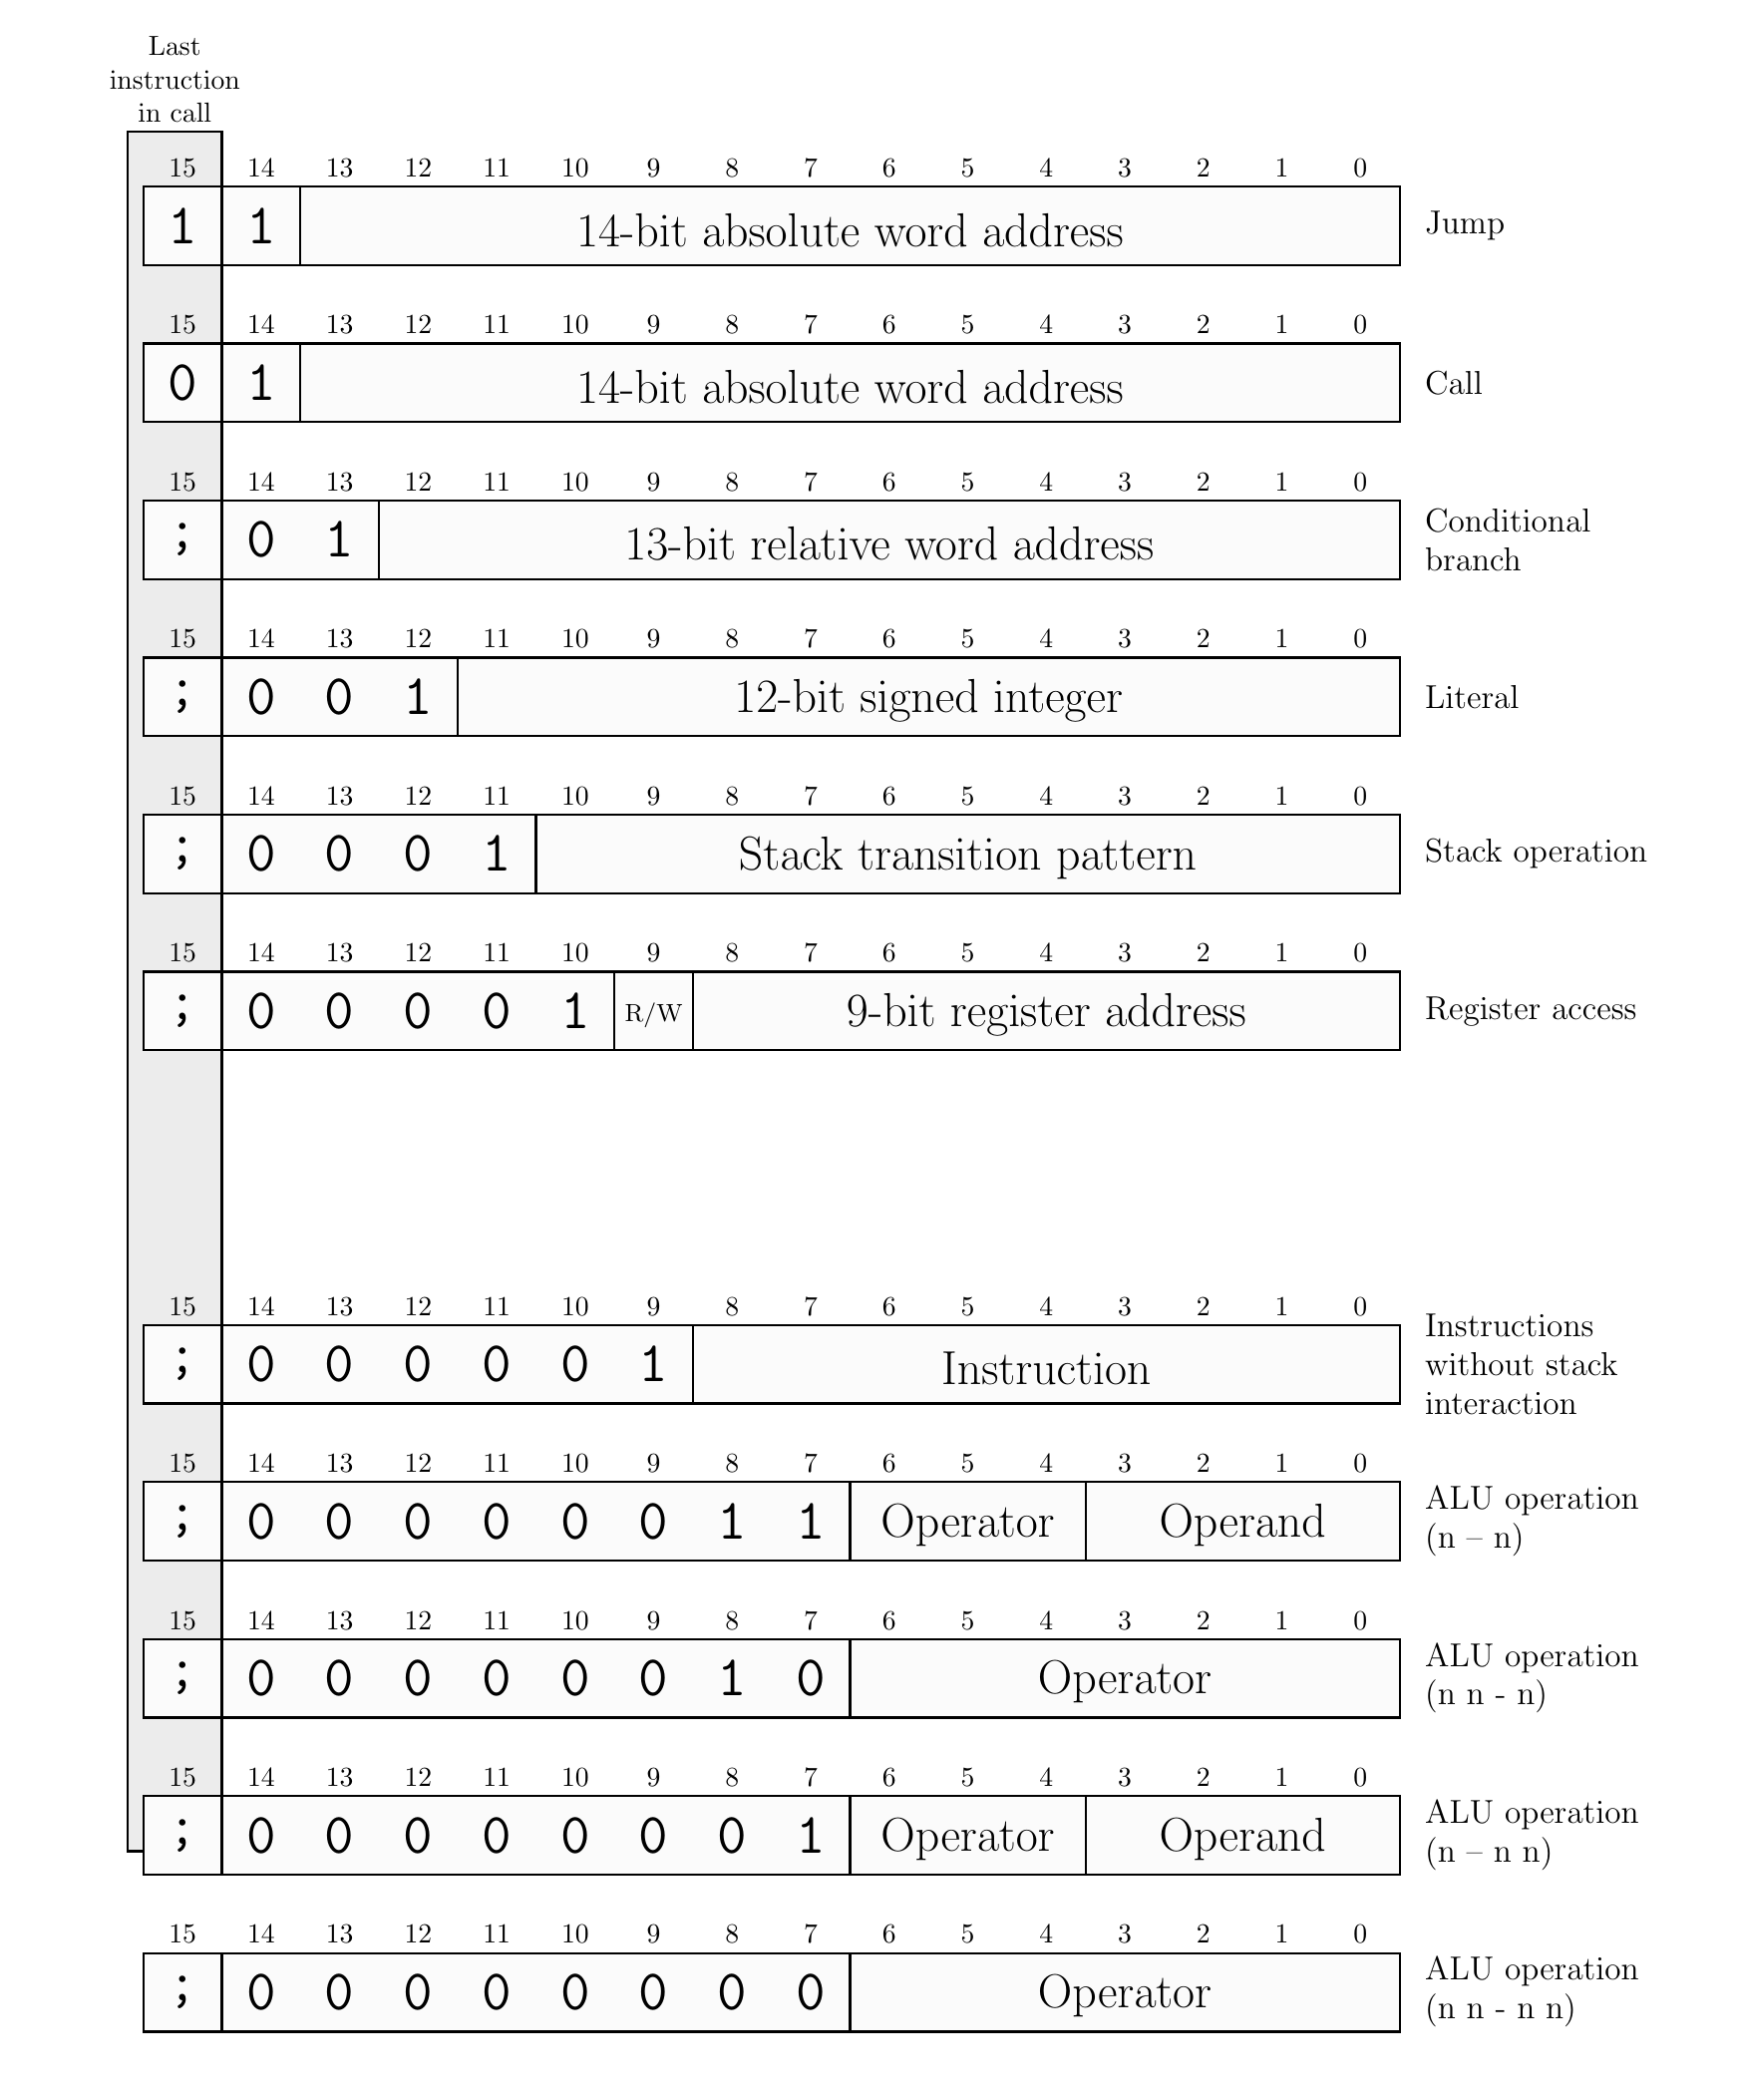
\begin{tikzpicture}
      
        %Instruction
        \newsavebox{\instruction}
        \savebox{\instruction}{
          \draw [thick, fill=gray!3] (0,0) rectangle (16,1);
          \draw [thick, fill=gray!3] (0,0) rectangle (1,1);
          \node [above] at (0.5,1)  {15};
          \node [above] at (1.5,1)  {14};
          \node [above] at (2.5,1)  {13};
          \node [above] at (3.5,1)  {12};
          \node [above] at (4.5,1)  {11};
          \node [above] at (5.5,1)  {10};
          \node [above] at (6.5,1)  {9};
          \node [above] at (7.5,1)  {8};
          \node [above] at (8.5,1)  {7};
          \node [above] at (9.5,1)  {6};
          \node [above] at (10.5,1) {5};
          \node [above] at (11.5,1) {4};
          \node [above] at (12.5,1) {3};
          \node [above] at (13.5,1) {2};
          \node [above] at (14.5,1) {1};
          \node [above] at (15.5,1) {0};
        };

        %Return bit
        \draw [thick, fill=gray!15] (0.8,2.8) rectangle (2,24.7);
        \node [above] at (1.4,24.7) {
          \begin{minipage}[c]{10em}
            \begin{center}
              Last \\
              instruction \\
              in call
            \end{center}
          \end{minipage}};
      
        %Jump
        \node at (1,23) {\usebox{\instruction}};
        \node         at (1.5,23.5)   {\huge{\texttt{1}}};
        \draw [thick] (2,23) rectangle (3,24);
        \node         at (2.5,23.5)   {\huge{\texttt{1}}};
        \node         at (10,23.45)   {\LARGE{14-bit absolute word address}};
        \node [right] at (17.2,23.5)  {\large{Jump}};
     
        %Call
        \node at (1,21) {\usebox{\instruction}};
        \node         at (1.5,21.5)   {\huge{\texttt{0}}};
        \draw [thick] (2,21) rectangle (3,22);
        \node         at (2.5,21.5)   {\huge{\texttt{1}}};
        \node         at (10,21.45)   {\LARGE{14-bit absolute word address}};
        \node [right] at (17.2,21.5)  {\large{Call}};
       
        %Conditional Branch
        \node at (1,19) {\usebox{\instruction}};
        \node         at (1.5,19.5)   {\huge{\texttt{;}}};
        \draw [thick] (2,19) rectangle (4,20); 
        \node         at (2.5,19.5)   {\huge{\texttt{0}}};
        \node         at (3.5,19.5)   {\huge{\texttt{1}}};
        \node         at (10.5,19.45) {\LARGE{13-bit relative word address}};
        \node [right] at (17.2,19.5)  {
          \begin{minipage}[l]{10em}
            \large{
              Conditional \\
              branch
            }
        \end{minipage}};
        
        %Literal 
        \node at (1,17) {\usebox{\instruction}};
        \node         at (1.5,17.5)   {\huge{\texttt{;}}};
        \draw [thick] (2,17) rectangle (5,18); 
        \node         at (2.5,17.5)   {\huge{\texttt{0}}};
        \node         at (3.5,17.5)   {\huge{\texttt{0}}};
        \node         at (4.5,17.5)   {\huge{\texttt{1}}};
        \node         at (11,17.45)   {\LARGE{12-bit signed integer}};
        \node [right] at (17.2,17.5)  {\large{Literal}};

        %Stack operation 
        \node at (1,15) {\usebox{\instruction}};
        \node         at (1.5,15.5)   {\huge{\texttt{;}}};
        \draw [thick] (2,15) rectangle (6,16); 
        \node         at (2.5,15.5)   {\huge{\texttt{0}}};
        \node         at (3.5,15.5)   {\huge{\texttt{0}}};
        \node         at (4.5,15.5)   {\huge{\texttt{0}}};
        \node         at (5.5,15.5)   {\huge{\texttt{1}}};   
        \node         at (11.5,15.45) {\LARGE{Stack transition pattern}};
        \node [right] at (17.2,15.5)  {\large{Stack operation}};
        
        %Register access
        \node at (1,13) {\usebox{\instruction}};
        \node         at (1.5,13.5)   {\huge{\texttt{;}}};
        \draw [thick] (2,13) rectangle (7,14); 
        \draw [thick] (7,13) rectangle (8,14); 
        \node         at (2.5,13.5)   {\huge{\texttt{0}}};
        \node         at (3.5,13.5)   {\huge{\texttt{0}}};
        \node         at (4.5,13.5)   {\huge{\texttt{0}}};
        \node         at (5.5,13.5)   {\huge{\texttt{0}}};   
        \node         at (6.5,13.5)   {\huge{\texttt{1}}};   
        \node         at (7.5,13.45)  {\small{R/\textoverline{W}}};   
        \node         at (12.5,13.45) {\LARGE{9-bit register address}};
        \node [right] at (17.2,13.5)  {\large{Register access}};

        %Control Instructions
        \node at (1,8.5) {\usebox{\instruction}};
        \node         at (1.5,9)       {\huge{\texttt{;}}};
        \draw [thick] (2,8.5) rectangle (8,9.5); 
        \node         at (2.5,9)       {\huge{\texttt{0}}};
        \node         at (3.5,9)       {\huge{\texttt{0}}};
        \node         at (4.5,9)       {\huge{\texttt{0}}};
        \node         at (5.5,9)       {\huge{\texttt{0}}};   
        \node         at (6.5,9)       {\huge{\texttt{0}}};   
        \node         at (7.5,9)       {\huge{\texttt{1}}};   
        \node         at (12.5,8.95)  {\LARGE{Instruction}};
        \node [right] at (17.2,9) {
          \begin{minipage}[l]{10em}
            \large{
              Instructions \\
              without stack \\
              interaction
            }
        \end{minipage}};
            
        %ALU operation (n -- n) 
        \node at (1,6.5) {\usebox{\instruction}};
        \node         at (1.5,7)      {\huge{\texttt{;}}};
        \draw [thick] (2,6.5) rectangle (10,7.5); 
        \draw [thick] (10,6.5) rectangle (13,7.5); 
        \node         at (2.5,7)      {\huge{\texttt{0}}};
        \node         at (3.5,7)      {\huge{\texttt{0}}};
        \node         at (4.5,7)      {\huge{\texttt{0}}};
        \node         at (5.5,7)      {\huge{\texttt{0}}};   
        \node         at (6.5,7)      {\huge{\texttt{0}}};   
        \node         at (7.5,7)      {\huge{\texttt{0}}};   
        \node         at (8.5,7)      {\huge{\texttt{1}}};   
        \node         at (9.5,7)      {\huge{\texttt{1}}};   
        \node         at (11.5,6.95)  {\LARGE{Operator}};
        \node         at (15,6.95)    {\LARGE{Operand}};
        \node [right] at (17.2,7) {
          \begin{minipage}[l]{10em}
            \large{
              ALU operation \\
              (n -- n)
            }
        \end{minipage}};
               
        %ALU operation (n n -- n) 
        \node at (1,4.5) {\usebox{\instruction}};
        \node         at (1.5,5)      {\huge{\texttt{;}}};
        \draw [thick] (2,4.5) rectangle (10,5.5); 
        \node         at (2.5,5)      {\huge{\texttt{0}}};
        \node         at (3.5,5)      {\huge{\texttt{0}}};
        \node         at (4.5,5)      {\huge{\texttt{0}}};
        \node         at (5.5,5)      {\huge{\texttt{0}}};   
        \node         at (6.5,5)      {\huge{\texttt{0}}};   
        \node         at (7.5,5)      {\huge{\texttt{0}}};   
        \node         at (8.5,5)      {\huge{\texttt{1}}};   
        \node         at (9.5,5)      {\huge{\texttt{0}}};   
        \node         at (13.5,4.95)  {\LARGE{Operator}};
        \node [right] at (17.2,5) {
          \begin{minipage}[l]{10em}
            \large{
              ALU operation \\
              (n n - n)
            }
        \end{minipage}};
            
        %ALU operation (n -- n n)
        \node at (1,2.5) {\usebox{\instruction}};
        \node         at (1.5,3)      {\huge{\texttt{;}}};
        \draw [thick] (2,2.5) rectangle (10,3.5); 
        \draw [thick] (10,2.5) rectangle (13,3.5); 
        \node         at (2.5,3)      {\huge{\texttt{0}}};
        \node         at (3.5,3)      {\huge{\texttt{0}}};
        \node         at (4.5,3)      {\huge{\texttt{0}}};
        \node         at (5.5,3)      {\huge{\texttt{0}}};   
        \node         at (6.5,3)      {\huge{\texttt{0}}};   
        \node         at (7.5,3)      {\huge{\texttt{0}}};   
        \node         at (8.5,3)      {\huge{\texttt{0}}};   
        \node         at (9.5,3)      {\huge{\texttt{1}}};   
        \node         at (11.5,2.95)  {\LARGE{Operator}};
        \node         at (15,2.95)    {\LARGE{Operand}};
        \node [right] at (17.2,3)   {
          \begin{minipage}[l]{10em}
            \large{
              ALU operation \\
              (n -- n n)
            }
        \end{minipage}};
               
        %ALU operation (n n -- n n)
        \node at (1,0.5) {\usebox{\instruction}};
        \node         at (1.5,1)      {\huge{\texttt{;}}};
        \draw [thick] (2,0.5) rectangle (10,1.5); 
        \node         at (2.5,1)      {\huge{\texttt{0}}};
        \node         at (3.5,1)      {\huge{\texttt{0}}};
        \node         at (4.5,1)      {\huge{\texttt{0}}};
        \node         at (5.5,1)      {\huge{\texttt{0}}};   
        \node         at (6.5,1)      {\huge{\texttt{0}}};   
        \node         at (7.5,1)      {\huge{\texttt{0}}};   
        \node         at (8.5,1)      {\huge{\texttt{0}}};   
        \node         at (9.5,1)      {\huge{\texttt{0}}};   
        \node         at (13.5,0.95)  {\LARGE{Operator}};
        \node [right] at (17.2,1) {
          \begin{minipage}[l]{10em}
            \large{
              ALU operation \\
              (n n - n n)
            }
        \end{minipage}};

      \end{tikzpicture}
    }
  }
  \caption{Instruction encoding}
  \label{opcodes:encoding}
  %\end{center}
\end{figure}

%\subsection{Address Region Descriptors}
%
%\begin{description}[style=nextline]
%  
%\item[\texttt{region\_adr\_i}] Target region descriptors (base addresses). \\
%  
%  The address range of each bus target is determined by a base address and an address mask.
%  An address \texttt{itr\_adr\_i} is within the range of the $n$-th bus target if 
%  \begin{center}
%    \texttt{itr\_adr\_i[ADR\_WIDTH-1:0] |
%      region\_msk\_i[(ADR\_WIDTH*($n$+1))-1:ADR\_WIDTH*$n$]} \\
%    $\equiv$ \\
%    \texttt{region\_adr\_i[(ADR\_WIDTH*($n$+1))-1:ADR\_WIDTH*$n$] |
%      region\_msk\_i[(ADR\_WIDTH*($n$+1))-1:ADR\_WIDTH*$n$]} \\
%  \end{center}
%
%\item[\texttt{region\_msk\_i}]  Target region descriptors (address masks). \\
%  See \texttt{region\_adr\_i}. 
%   
%\end{description}
